\documentclass[12pt,a4paper]{article}
\usepackage[margin=2.5cm]{geometry}
\usepackage{amsmath,amssymb,graphicx,setspace,palatino,float,subcaption, booktabs, titlesec,lineno}
\usepackage[colorlinks, allcolors = blue]{hyperref}
\usepackage{natbib}
\citestyle{egu}

\usepackage[section]{placeins}
\usepackage[usenames,dvipsnames]{xcolor}

\captionsetup[figure]{labelfont=bf,textfont={small,normalfont}}
%\captionsetup[subfigure]{labelsep=quad, labelfont={bf,small}, textfont=small, singlelinecheck=off, justification=raggedright, position=top}
%\renewcommand{\thesubfigure}{\Alph{subfigure}}

\renewcommand{\subsectionautorefname}{Section}
\renewcommand{\subsubsectionautorefname}{Section}
\titleformat{\paragraph}[hang]{\normalfont\normalsize\itshape}{\theparagraph}{0em}{}
\titlespacing*{\paragraph}{0pt}{1\baselineskip}{3pt}
\setlength{\parindent}{0pt}
\setlength{\parskip}{\baselineskip}

\renewcommand{\subsectionautorefname}{Methods section}
\renewcommand{\subsubsectionautorefname}{Methods section}
\renewcommand{\thesubsection}{\arabic{subsection}}

\newcommand{\cmnt}[1]{{\color{purple} #1}}

\title{Antisense transcripts can quickly evolve to encode proteins}
\author{Bharat Ravi Iyengar$^{1,\dagger}$, Erich Bornberg-Bauer$^{1,2}$}
\date{\small $^1$Institute for Evolution and Biodiversity, University of M\"{u}nster,\\ H\"{u}fferstrasse 1, 48149 M\"{u}nster, Germany\\[1ex] $^2$Department of Protein Evolution, Max Planck Institute for Biology T\"{u}bingen, Max-Planck-Ring 5, 72076 T\"{u}bingen, Germany \\[1ex] $^\dagger$ Corresponding author: b.ravi@uni-muenster.de}

\begin{document}

\onehalfspacing
\def\figdir{../Figures/M2_main/pdf}

\setlength{\abovedisplayskip}{0pt}
\setlength{\belowdisplayskip}{1em}

\maketitle


\linenumbers

\section*{Abstract}




\section*{Introduction}



\section*{Results}

We developed mathematical models to estimate the probabilities of ORF emergence and loss, in DNA regions antisense to existing protein coding ORFs. These models are defined by two kinds of probability. The first is the probability of finding a certain kind of DNA sequence, for example an ORF. This stationary probability depends on the nucleotide composition of the DNA region that can be roughly approximated by GC-content or by the frequencies of short DNA sequences (k-mers). The second kind of probability describes the mutational change of a sequence to a different kind of sequence. For example, gain or loss of an ORF. This transition probability depends on the mutation rate and mutation bias, in addition to nucleotide composition. We estimate these parameters primarily from the data on the yeast, \textit{Saccharomyces cerevisiae} \citep{scermutrate}. Our choice is motivated by the fact that yeast is a convenient model organism for laboratory experimental studies that can be used to validate theoretical predictions. We also perform analogous analyses using data obtained from \textit{Drosophila melanogaster} \citep[][Supplementary section XX]{drosophilamutrate}.

We estimate the stationary and transition probabilities of antisense ORFs using the existing (sense) ORF as a reference. Specifically, we analyse the effect of the composition of the sense ORF, and of mutations in its sequence, to determine how likely it is for an antisense ORFs to exist, and to be gained or lost. Antisense ORFs can overlap with the sense ORFs in three different frames. In frame 0, the codons in the antisense ORF exactly overlap the codons in the sense ORF. In frames 1 and 2, the codons in the antisense ORF are shifted towards the 5' end of the sense ORF by one and two nucleotide positions, respectively. Thus in frames 1 and 2, the sequence of an antisense codon is determined by two partially overlapping sense codons (dicodons). Due to this sequence overlap, the evolution of antisense ORFs would be constrained by the evolutionary selection pressures on the sense ORF. Furthermore, these constraints would be different for antisense ORFs located in the three different frames. We analysed the evolution of antisense ORFs when the sense ORF is under three different levels of purifying selection. The first level describes an absence of purifying selection, where any kind of mutation except a non-sense mutation (gain of stop codon) in the sense ORF is tolerated. The second level describes a weak purifying selection that allows synonymous mutations (nucleotide mutations that do not change the encoded amino acid), as well as mutations where an amino acid is substituted by a chemically similar amino acid (for example, aspartic acid to glutamic acid). Finally, in the third level that describes a strong purifying selection, only synonymous mutations are tolerated in the sense ORF.

\subsection*{Antisense ORFs are more likely to exist in frame 1}

For any stretch of DNA to be an ORF, its sequence should contain 3$n$ nucleotides (with $n$ being at least 3), with a start codon that marks its beginning, and exactly one stop codon that marks its end. The absence of any stop codon within the DNA sequence is the most important factor in determining the existence of an ORF. That is because the likelihood of a premature stop codon increases exponentially with the ORF's length, whereas the likelihoods of a start codon and a terminal stop codon are independent of the ORF's length. Furthermore, overlapping DNA region between the sense and antisense ORF would mostly consist of non-terminal (internal) codons. 

\begin{figure}[!t]
\centering
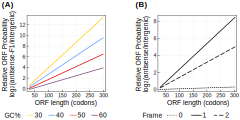
\includegraphics[scale=0.5]{\figdir/pORF_antisense_scer.pdf}
\caption{Antisense ORFs in frame 1 are more likely to exist than intergenic ORFs of identical lengths. Panel \textbf{(A)} shows the probability of antisense ORFs in frame 1 relative to that of intergenic ORFs ($\log_2$ ratio, vertical axis). Line colors indicate the GC-content of the ORFs (yellow = 30\%, blue = 40\%, red = 50\%, purple = 60\%). We do not show antisense ORFs in frames 0 and 2 because their probabilities are identical to that of intergenic ORFs. Panel \textbf{(B)} shows the probability of antisense ORFs relative to that of intergenic ORFs ($\log_2$ ratio, vertical axis), calculated using frequencies of short DNA sequences from the yeast genome. Frames 0, 1 and 2 are denoted by dotted, solid and dashed lines, respectively. Horizontal axis in both panels shows the length of the ORFs. For data in both panels, we assume that antisense ORFs overlap completely with the sense ORF.}
\label{pORF}
\end{figure}

Based on these considerations, we determined the probability of finding an antisense ORF. To this end, we calculated the probability of finding a stop codon in the three antisense frames, given the nucleotide composition of the sense ORF, including the condition that no stop codon exists in the sense ORF. Specifically, a stop codon can exist in frame 0 wherever the reverse complementary codons (\texttt{TTA},\texttt{CTA},\texttt{TCA}) exist in the sense ORF. It can exist in frames 1 and 2, overlapping with one of the 128 and 192 dicodons in the sense ORF, respectively. We next calculated the probability of an antisense stop codon based on the probability of the corresponding sense codons and dicodons. We calculated the probability of finding a start codon using the general GC-content of the locus, ignoring any effect of the sense ORF. Using the start and stop codon probabilities, we estimated the probability of finding an antisense ORF of different lengths in each of the three frames. We did so for four different values of GC-content. We found that frame 1 has the highest likelihood of harboring an antisense ORF in 99.2\% of cases. The only exceptions are ORFs shorter than 39 codons present in a DNA region with a GC-content of 60\%. Even for these exceptional cases, the probability of an antisense ORF in frame 1 is no less than 91\% of the corresponding ORF probabilities in the other frames. 

To understand whether antisense ORFs are more likely to be found than ORFs in intergenic regions, we compared the probabilities of antisense ORFs with that of intergenic ORFs of identical GC-content and lengths. We note that that the probability of intergenic ORFs is not constrained by existing ORFs and is thus purely dependent on nucleotide composition. We found that the probability of antisense ORFs in frames 0 and 2 were identical to that of the corresponding intergenic ORFs, which means that antisense ORFs in frame 1 are more likely to exist than intergenic ORFs except in the 0.8\% cases where the ORFs have a GC-content of 60\% and less than 39 codons. 

GC-content may not accurately describe the nucleotide composition of a locus. Therefore, we also calculated the probability of antisense ORFs using actual codon and dicodon frequencies in yeast ORFs. Likewise, we calculated the probability of intergenic ORFs using the frequencies of DNA trimers in yeast intergenic genome. With this analysis, we found that antisense ORFs longer than 54 and 75 codons in frames 1 and 2, respectively, are more likely to exist than intergenic ORF of the same lengths. For all ORF lengths, antisense ORFs in frame 3 are less likely to exist than intergenic ORFs. 

Our complementary analyses using \textit{D. melanogaster} as a model for mutation bias, produced similar results. However, when we computed the ORF probabilities using the frequencies of codons, dicodons and intergenic trimers from  \textit{D. melanogaster}, we found that frame 0 was most likely to harbor an antisense ORF. 

\subsection*{Antisense overlap can facilitate ORF emergence and reduce ORF loss}

\begin{figure}[!b]
\centering
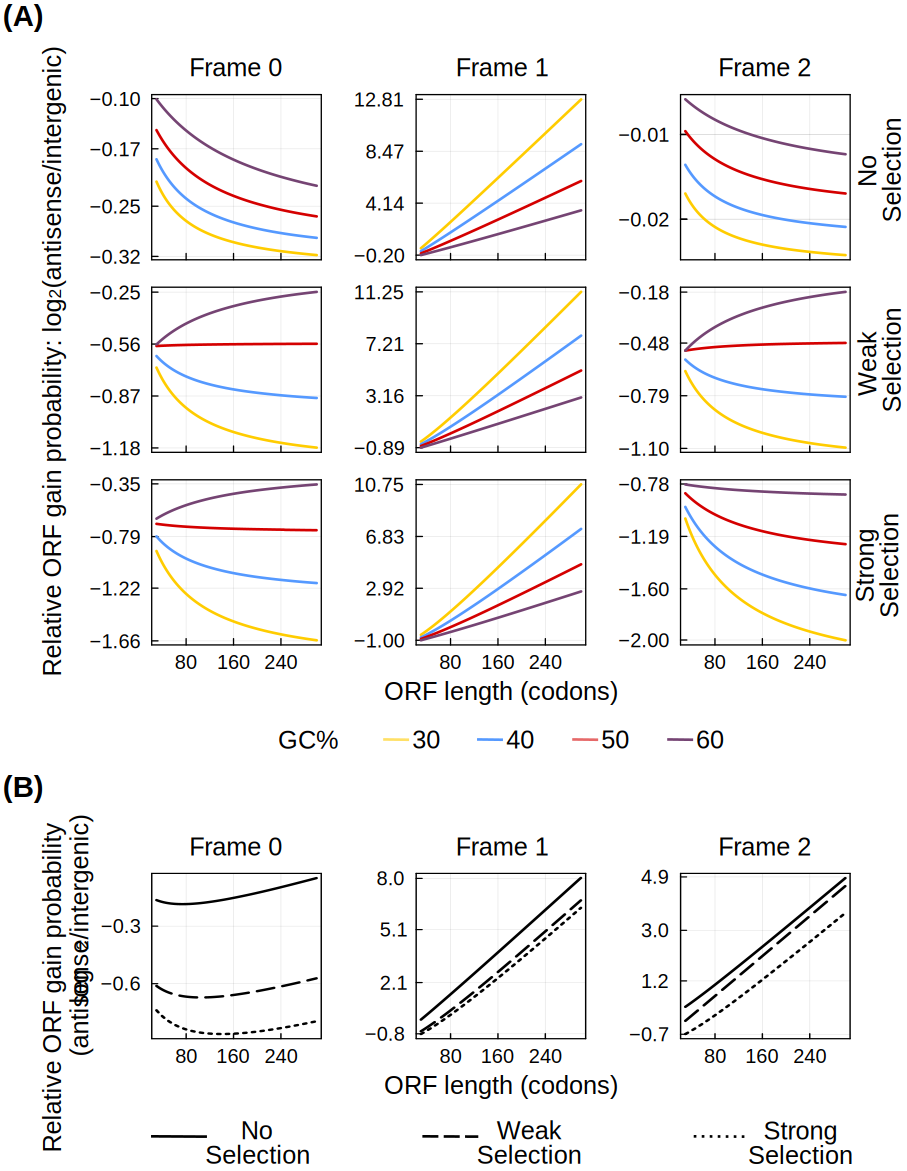
\includegraphics[scale=0.5]{\figdir/pORFgain_antisense_scer.pdf}
\caption{Antisense overlap can facilitate ORF emergence. Panel \textbf{(A)} shows the probability of ORF emergence in the three antisense frames (left to right) relative to that in intergenic regions ($\log_2$ ratio, vertical axis), at different intensities of purifying selection (top to bottom). Line colors indicate the GC-content of the ORFs. Panel \textbf{(B)} shows the ORFs gain probability in the three antisense frames relative to that in intergenic regions ($\log_2$ ratio, vertical axis), calculated using frequencies of short DNA sequences from the yeast genome. Dotted, solid and dashed lines, denote the zero, weak and strong purifying selection, respectively. Horizontal axis in all panels shows the length of the ORFs. For data in both panels, we assume that antisense ORFs overlap completely with the sense ORF.}
\label{pORFgain}
\end{figure}

We next analysed how likely it is for antisense ORFs to emerge, when they are not already present. To this end, we calculated gain probability of antisense ORFs in each of the three frames, and under three different intensities of purifying selection. We also calculated the probability of ORF gain in the intergenic regions. We found that antisense ORFs are less likely to emerge in frames 0 and 2, than ORFs in intergenic regions, for all ORF lengths and GC-content. In contrast, the emergence of antisense ORF emergence in frame 1 is often more likely than that of intergenic ORFs, especially when the ORFs are long. 



Increasing the intensity of purifying selection, reduces the emergence likelihood of antisense ORFs in all three frames. However, emergence of antisense ORFs in frame 1 is still more likely than emergence of intergenic ORFs, even under strong purifying selection. Specifically, the minimum ORF length where frame 1 antisense ORFs are more likely to emerge than intergenic ORFs, increases with GC-content and the intensity of selection. For example, in the absence of purifying selection and a GC-content of 30\%, this length is smaller than the smallest investigated ORF length of 30 codons. At the same intensity of selection, this length is 46 codons when the GC-content is 60\%. ORFs can emerge in antisense frame 1 more frequently than in intergenic regions under strong purifying selection, with GC-contents of 30\% and 60\%, if they are longer 49 and 109 codons, respectively.

\begin{figure}[!b]
\centering
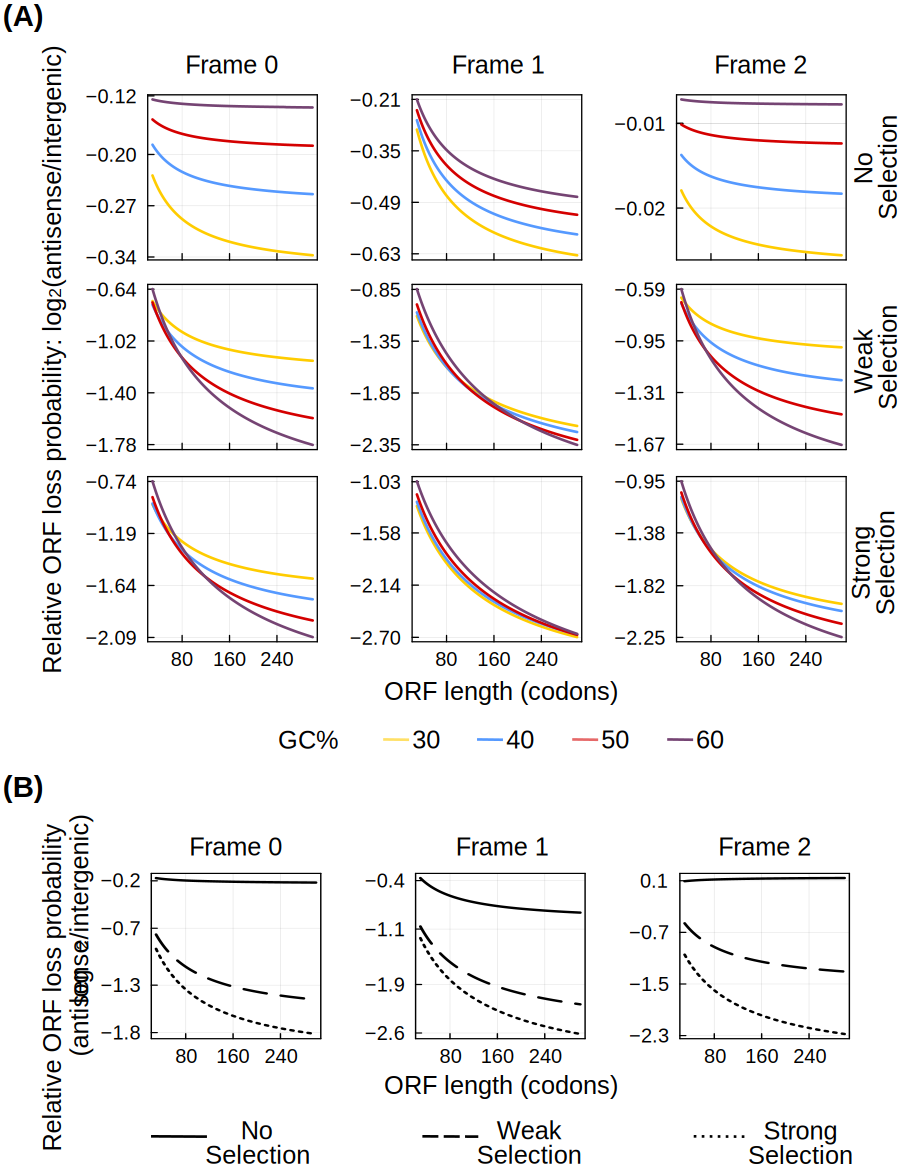
\includegraphics[scale=0.5]{\figdir/pORFloss_antisense_scer.pdf}
\caption{Antisense overlap can reduce ORF loss. Panel \textbf{(A)} shows the probability of ORF loss in the three antisense frames (left to right) relative to that in intergenic regions ($\log_2$ ratio, vertical axis), at different intensities of purifying selection (top to bottom). Line colors indicate the GC-content of the ORFs. Panel \textbf{(B)} shows the ORFs loss probability in the three antisense frames relative to that in intergenic regions ($\log_2$ ratio, vertical axis), calculated using frequencies of short DNA sequences from the yeast genome. Dotted, solid and dashed lines, denote the zero, weak and strong purifying selection, respectively. Horizontal axis in all panels shows the length of the ORFs. For data in both panels, we assume that antisense ORFs overlap completely with the sense ORF.}
\label{pORFloss}
\end{figure}

Our analysis of ORF gain probabilities using the frequencies of DNA oligomers (codons, dicodons and intergenic trimers), also shows that antisense ORFs are very likely to emerge in frame 1. ORFs longer than 30 (shortest investigated length), 60 and 69 codons are more likely to emerge in antisense frame 1 than in intergenic regions, when the purifying selection is absent, weak and strong, respectively. Interestingly, this analysis revealed that although antisense ORFs are less likely to emerge in frame 2 than in frame 1, they can emerge more frequently than intergenic ORFs. Specifically when the purifying selection is absent, weak and strong, ORFs that are more likely to emerge in antisense frame 2 than in intergenic regions, contain at least 30, 43 and 82 codons, respectively.


Purifying selection reduces the number of tolerated mutations in a DNA locus. We note again that our lowest level of purifying selection also disallows nonsense mutations from occurring in the sense ORFs. We thus hypothesized that overlap with a sense ORF may protect the antisense ORFs from being lost. To this end, we calculated ORF loss probabilities for different ORF lengths, GC-content, and intensities of purifying selection. In an analogous analysis, we used codon, dicodon, and intergenic trimer frequencies, instead of GC-content, to calculate ORF loss probabilities. Our analyses show that antisense ORFs are indeed protected from loss due to overlap with existing ORFs. That is, the loss probability of antisense ORFs is less than that of intergenic ORFs. This protection against loss increases with increasing intensity of purifying selection. However, selection does not protect the ORFs in all the three antisense frames equally. Antisense ORFs are more likely to be preserved when they exist in frame 1. 

Overall, our analyses suggest that antisense overlap with an existing ORF facilitates emergence of new ORFs, and protects the existing antisense ORFs from being lost. A complementary analysis with parameters estimated from \textit{D. melanogaster} further supports this finding.

\subsection*{Overlap with sense ORFs promotes divergence of antisense ORFs in frame 2}

In the previous sections, we showed that purifying selection on the sense ORF can affect the emergence and loss of antisense ORFs. We next asked if this purifying selection can also constrain the diversification of the proteins encoded by antisense ORF sequences. To this end, we first calculated the chemical distance ($\delta$) between any two amino acids. For this calculation we used a distance matrix that we derived from an experimentally estimated amino acid similarity matrix reported in a previous study \citep{PMBEC}. Next, we calculated the average chemical difference ($\bar{\delta}$) introduced by a random mutation, weighted by the probability of different mutations. Using $\bar{\delta}$ as a measure of divergence, we estimated the extent to which antisense ORFs in the three frames, can diverge as a result of mutations, and due to purifying selection on the sense ORFs. Likewise, we also calculated the divergence of intergenic ORFs as a consequence of random mutations. 

We found that frame 2 allows maximum divergence of antisense ORFs, under both weak and strong purifying selection on the sense ORF. Antisense ORFs in frame 0 diverge the least. Interestingly, strong selection on sense ORF increases the divergence of antisense ORFs in frame 2. The reason could be that the few mutations that do occur under strong purifying selection, cause a relatively higher increase in divergence than the more numerous mutations that are allowed to occur under weak purifying selection. We also found that the divergence of frame 2 antisense ORFs was higher than than that of intergenic ORFs under both selection regimes. We note this result does not mean that intergenic ORFs can diverge less than antisense ORFs. Evolution of intergenic ORFs is not constrained by another DNA sequence. However, as long as the mutants do not affect the organismal fitness, evolution would not be biased towards divergence increasing mutations. Thus random mutations in intergenic ORFs could also consist of many synonymous and chemistry preserving mutations, that are probably disallowed in frame 2 antisense ORFs due to purifying selection on sense ORFs.

In contrast to frame 2, the divergence of antisense ORFs in the other two frames decreased with increasing strength of purifying selection on the sense ORF. For example, frame 0 antisense ORFs did not diverge at all when the sense ORF was under strong purifying selection. Antisense ORFs in frames 0 and 1 also diverged less than intergenic ORFs under both selection regimes. 


\begin{figure}[!t]
\centering
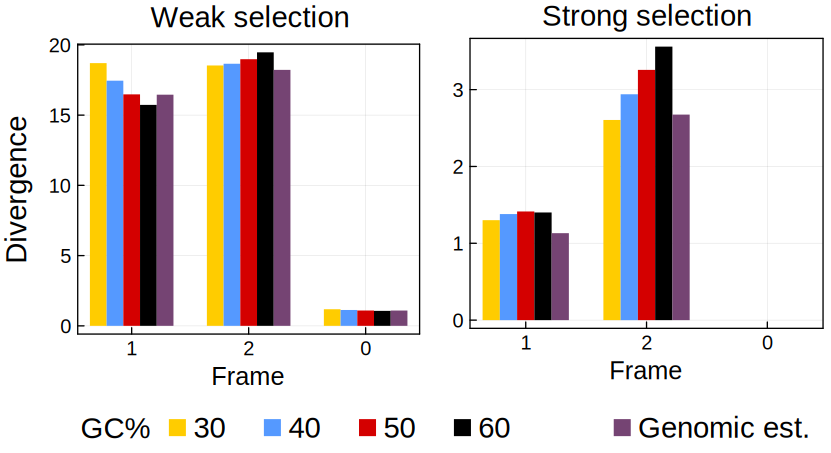
\includegraphics[scale=0.5]{\figdir/Divergence_scer.pdf}
\caption{Antisense ORFs can diversify when sense ORFs are under purifying selection. Vertical axis denotes the divergence ($\bar{\delta}$) of antisense ORFs due to a random mutation when the sense ORF is under weak (left) or strong (right) purifying selection. Horizontal axes denote the three antisense frames. Colored bars denote divergence values of antisense ORFs with different GC-content, and black bars denote the diversity values calculated using frequencies of short DNA sequences from the yeast genome. Filled circles that are similarly color coded, denote the divergence of intergenic ORFs due to mutations.}
\label{divergence}
\end{figure}
\section*{Discussion} 


\section*{Materials and Methods}

\subsection{Mutation probabilities}

\begin{table}[H]
\centering
\begin{tabular}{c c}
\toprule
\textbf{Substitution} & Probability($\mu$) \\\midrule
\texttt{A:T}$\to$\texttt{T:A} & 0.056 \\\midrule
\texttt{A:T}$\to$\texttt{G:C} & 0.243 \\\midrule
\texttt{A:T}$\to$\texttt{C:G} & 0.074 \\\midrule
\texttt{G:C}$\to$\texttt{A:T} & 0.483 \\\midrule
\texttt{G:C}$\to$\texttt{T:A} & 0.075 \\\midrule
\texttt{G:C}$\to$\texttt{C:G} & 0.069 \\\bottomrule
\end{tabular}
\caption{Mutation bias probabilities for different nucleotide mutations. \texttt{A:T} denotes an \texttt{A}-\texttt{T} base pair in a double stranded DNA. Thus \texttt{A}$\to$\texttt{G} mutation on one DNA strand would cause a \texttt{T}$\to$\texttt{C} mutation on the complementary strand. We describe the other mutations in the same way.}
\label{mutbias}
\end{table}




%\subsection{Probabilities of finding, gaining, and losing a DNA sequence}
%\label{methbasic}
%
%\subsubsection{Probability of finding a DNA sequence}
%\label{methprob}
%
%We calculated the probability of finding a DNA sequence based on global nucleotide frequency distributions, given by the GC-content. Specifically, the probability of finding either a \texttt{G} or a \texttt{C} is: 
%
%$$S = \frac{0.5\times\text{GC\%}}{100}$$
%
%The probability of finding an \texttt{A} or a \texttt{T} is: $W = 0.5 - S$. Using these values, we calculated the probability of finding a DNA sequence motif by chance. For example, the probability of finding the sequence \texttt{ATG} would be: $W\times W \times S$.
%
%\cmnt{We also estimated the probability of finding specific DNA sequences in a reference genome. Specifically, we calculated the frequencies of all 64 trimers and all 4096 hexamers in the genomic regions of \textit{D. melanogaster} that exist in open chromatin, and do not contain any known genes or regulatory elements (see \autoref{methRNA})}.
%
%\subsubsection{Probability of gaining a DNA sequence}
%\label{methgain}
%
%We calculated the probability of gaining a DNA sequence due to mutations using GC-content, mutation rate and mutation bias. Specifically, we calculated the probability that a DNA sequence does not exist, and it emerges due to specific nucleotide mutations. More precisely, this probability is the product of two other probabilities. The first is the probability of finding a DNA sequence ($x$) that is not the sequence of interest. The second probability is that this sequence $x$ mutates to the sequence of interest. To explain this calculation better, we use the example of \texttt{CTA} mutating to \texttt{ATG}. The first probability, that is the probability of finding \texttt{CTA} by chance is $SW^2$. \texttt{CTA} mutates to \texttt{ATG} via two nucleotide mutations (\texttt{C}$\to$\texttt{A} and \texttt{A}$\to$\texttt{G}). Thus the probability of this DNA change would be the probability of two nucleotide mutations ($\lambda^2$) multiplied by two mutation bias probabilities (\texttt{G:C}$\to$\texttt{T:A} and \texttt{A:T}$\to$\texttt{G:C}). Overall, the chance of \texttt{CTA} mutating to \texttt{ATG} would be:
%
%$$SW^2 \times \lambda^2 \times \mu_{\texttt{G:C}\to\texttt{T:A}} \times \mu_{\texttt{A:T}\to\texttt{G:C}}$$
%
%Next, we calculated the probability that every nucleotide triplet that is not \texttt{ATG}, mutates to \texttt{ATG}. This can happen via one, two, or three nucleotide mutations. The sum of all these mutation probabilities is the probability of \texttt{ATG} gain.
%
%Using the same principle we calculated the gain probability of any DNA sequence motif (of any length or composition). We excluded insertions and deletions as a mechanism of gain of small DNA sequences that we analysed in this study. 
%
%
%\subsubsection{Probability of losing a DNA sequence}
%
%We calculated the loss of a DNA sequence motif using the same principle we used for calculating gain probabilities. However, we defined loss probability as a conditional probability, that is we assume that the DNA sequence of interest already exists in the genome. For example, the loss probability of a specific \texttt{ATG} sequence would be the sum of probabilities of \texttt{ATG} mutating to any of the other 63 nucleotide triplets (via one, two, or three nucleotide mutations). We use conditional loss probabilities by default, because usually one is interested in finding out how quickly an existing DNA sequence can erode.
%
%We used this method to calculate the loss probability of any DNA sequence motif, and we excluded insertions and deletions from this calculation.
%
%\subsection{Probabilities of finding, gaining, and losing DNA features}
%\label{methfeatures}
%
%Usually, a specific function is encoded in DNA by several DNA sequences. For example, translation stop is encoded by three codons (\texttt{TGA}, \texttt{TAG}, \texttt{TAA}). We use the term DNA features to mean a set of DNA sequences that are associated with the same function. For every such DNA feature set, there is a complementary set of non-features, that is DNA sequences that are not associated with the feature's function. For example, the non-feature set of stop codons would be all the other 61 codons. 
%
%The probability that a DNA feature exists, is the sum of probabilities of every DNA sequence in that set (\autoref{methprob}).
%
%The probability that a DNA feature is gained via mutations, is the sum of probabilities of every non-feature sequence mutating to any feature sequence. If $F$ denotes the feature set, and $\mu_{y\to x}$ denotes the probability of a DNA sequence $y$ mutating to a DNA sequence $x$ (see \autoref{methgain}), then:
%
%\begin{equation}
%P_\textit{feature-gain} = \sum_{x \in F} \sum_{y \notin F} P_y \times \mu_{y\to x}
%\end{equation}
%
%The probability that a DNA feature is lost via mutations is a conditional probability that given a feature exists, it mutates to any of the non-feature sequences. 
%
%\begin{equation}
%P_\textit{feature-loss} = \frac{\displaystyle\sum_{x \in F} \sum_{y \notin F} P_x \times \mu_{x\to y}}{\displaystyle\sum_{x \in F} P_x}
%\end{equation}
%
%Because a feature set usually has many DNA sequences, a mutation can change a feature sequence such that the resulting sequence is also a part of the feature set. Thus we defined the probability ($P_\textit{feature-stay}$) that a feature does not erode because of mutations. Specifically, it is the sum of two probabilities. First is the probability that no mutation occurs in the DNA sequence ($P_0$), and the second probability describes the event where the mutated sequence remains a part of the feature set.
%
%\begin{equation}
%P_\textit{feature-stay} = P_0 + \sum_{x \in F} \sum_{\genfrac{}{}{0pt}{1}{y \in F}{y\neq x}} \mu_{x\to y}
%\end{equation}
%
%
%The probability that no mutation occurs ($P_0$) in a DNA sequence of length $k$ is described by Poisson distribution. 
%
%$$P_0 = 1-e^{-k\lambda}$$
%
%Because the mutation rate is biased (\autoref{mutbias}), the probability that no mutation occurs in a DNA sequence depends on its composition. 
%
%The probability that an \texttt{A} or a \texttt{T} mutates ($\lambda_\texttt{AT}$), is thus described as:
%
%$$\lambda_\texttt{AT} = 2\times\lambda\times(\mu_{\texttt{A:T}\to\texttt{T:A}} + \mu_{\texttt{A:T}\to\texttt{G:C}} + \mu_{\texttt{A:T}\to\texttt{C:G}})$$
%
%Likewise, the probability that a \texttt{G} or a \texttt{C} mutates ($\lambda_\texttt{GC}$) is: 
%
%\vspace{-1ex}
%
%$$\lambda_\texttt{GC} = 2\times\lambda\times(\mu_{\texttt{G:C}\to\texttt{A:T}} + \mu_{\texttt{G:C}\to\texttt{T:A}} + \mu_{\texttt{G:C}\to\texttt{C:G}})$$
%
%(Note that the general mutation rate, $\lambda$, is an average of $\lambda_\texttt{AT}$ and $\lambda_\texttt{GC}$.)
%
%\vspace{1\baselineskip}
%
%Thus the probability that a sequence of length $k$, containing $m$ number of \texttt{A} and \texttt{T}, does not mutate is:
%
%\vspace{-1ex}
%
%$$P_0 = (1-e^{-m\lambda_\texttt{AT}})\times(1-e^{-(k-m)\lambda_\texttt{GC}})$$
%
%
%\cmnt{We also calculated all the above-defined probabilities ($P_\textit{feature-gain}$, $P_\textit{feature-loss}$ and $ P_\textit{feature-stay}$), using DNA trimer and hexamer frequencies from \textit{D. melanogaster}. In this case the probability of finding a nucleotide sequence depends on the trimer/hexamer distributions instead of GC-content, but the probability of mutational changes are only dependent on mutation bias. Trimers and hexamers would contain codons and polyA signals, respectively.}
%


\subsection{Probabilities of finding, gaining, and losing an ORF}

\label{methORF}

\subsubsection{Probability of finding an ORF}

A reading frame is a nucleotide sequence with a length that is a multiple of three. A reading frame that begins with a start codon (\texttt{ATG}), and ends with one of the three stop codons (\texttt{TAG}, \texttt{TGA}, \texttt{TAA}) is an open reading frame (ORF). This necessarily means that there are no stop codons within the sequence. Thus the probability of finding an ORF containing $k$ codons including start and stop codons ($P_\textit{ORF}$) is: 

\begin{equation}
P_\textit{ORF}(k) = P_\textit{ATG} \times P_\textit{stop} \times (1 - P_\textit{stop})^{k-2}
\label{eqorfprob}
\end{equation}

Here, $P_\textit{ATG}$ and $P_\textit{stop}$ are the probabilities of finding a start codon, and a stop codon by chance, respectively.

\subsubsection{Probability of gaining an ORF}

As we defined in the previous section, an ORF has three requirements (start codon, stop codon, and no premature stop codon in the sequence). Thus an ORF can emerge due to mutations via three mechanisms. In each of these mechanisms, one requirement is initially absent whereas the other two are present. Then mutations cause the missing requirement to emerge while not disrupting the other two requirements. More specifically, the ORF can be gained via the following three mechanisms:
\begin{enumerate}
\item Gain of a start codon ($P_\textit{ATG-gain}$) while a stop codon continues to exist at the end of a reading frame ($P_\textit{stop-stay}$), and there is no emergence of stop codon within the reading frame ($1- P_\textit{stop} - P_\textit{stop-gain}$).
\item Gain of a stop codon ($P_\textit{stop-gain}$), while a start codon continues to exist at the beginning of a reading frame ($P_\textit{ATG-stay}$), and there is no emergence of stop codon within the reading frame.
\item Loss of a premature stop codon, at any of the $k-2$ codon positions within the reading frame ($P_\textit{stop-gain}$). At the same time start and stop codons remain undisrupted by mutations, and no stop codon emerges at any of the other $k-3$ positions.
\end{enumerate} 

Thus we define the probability of ORF gain ($P_\textit{ORF-gain}$) as:

\begin{align}
P_\textit{ORF-gain}(k) & = \quad P_\textit{ATG-gain}\times P_\textit{stop-stay} \times (1- P_\textit{stop} - P_\textit{stop-gain})^{k-2} \nonumber \\[1pt]
& \quad + P_\textit{ATG-stay}\times P_\textit{stop-gain} \times (1- P_\textit{stop} - P_\textit{stop-gain})^{k-2} \nonumber \\[1pt]
& \quad + P_\textit{ATG-stay}\times P_\textit{stop-stay} \times P_\textit{stop-loss}\times(k-2) \times (1- P_\textit{stop} - P_\textit{stop-gain})^{k-3} 
\label{eqorfgain}
\end{align}

\subsubsection{Probability of ORF loss}

ORF can be lost when any of its three requirements are lost. We thus define the conditional probability of ORF loss as:

\begin{equation}
P_\textit{ORF-loss}(k) = P_\textit{ATG-loss} + P_\textit{stop-loss} + (k-2)\times \frac{P_\textit{stop-gain}}{1-P_\textit{stop}}
\label{eqorfloss}
\end{equation}

The last term in this equation describes the conditional probability of stop-gain, given the assumption that no stop codon exists within the ORF.

\subsubsection{Probability that ORF remains intact}

We assumed that an ORF of a certain length remains intact if none of the necessary features are lost. However, the ORF sequence can mutate to cause non-synonymous changes in the translated protein sequence. This condition applies to all the three ORF probabilities described above. We define the probability that an ORF remains intact ($P_\textit{ORF-stay}$) as:

\begin{equation}
P_\textit{ORF-stay}(k) = P_\textit{ATG-stay} \times P_\textit{stop-stay} \times (1 - P_\textit{stop} - P_\textit{stop-gain})^{k-2}
\label{eqorfstay}
\end{equation}

\subsection{Divergence of protein sequence}
Specifically, if $i$ denotes the original codon, $j$ denotes the substituted codon, $P_i$ denotes the probability of finding codon-$i$, $\mu_{ij}$ denotes the probability of codon-$i$ mutating to codon-$j$, and $\delta_{ij}$ denotes the chemical difference between the amino acids encoded by these codons, then the average chemical difference is defined by the following equation:

\begin{equation}
\bar{\delta} = \frac{\displaystyle\sum_i P_i \sum_j \mu_{ij}\delta_{ij}}{\displaystyle\sum_i P_i \sum_j \mu_{ij}}
\end{equation}


\section*{Data availability}
We performed all calculations using Julia programming language, and all scripts are freely available on GitHub: BharatRaviIyengar/DeNovoEvolution. Specifically, our model uses the following scripts:

\vspace{-2em}
\begin{itemize}\setlength{\itemsep}{-1pt}
\item \texttt{antisenseGenes.jl} (main script)
\item \texttt{antisenseGenes\_supplement.jl} \\(calculations using codon, dicodon, and intergenic trimer frequencies)
\item \texttt{nucleotidefuncts.jl} (dependency for basic functions)
\end{itemize}

\section*{Acknowledgments}

\bibliographystyle{mybst}

\small
\bibliography{refs}

\end{document}
